\documentclass{standalone}
\usepackage{tikz}
\usepackage{ctex}
\usepackage{xcolor}
\usetikzlibrary{3d}

\begin{document}


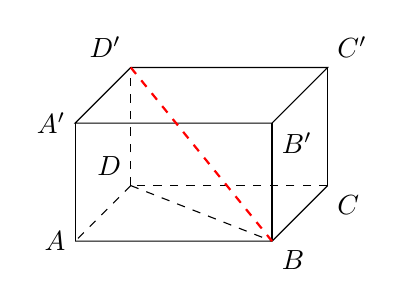
\begin{tikzpicture}[scale=0.5,
    y={(-0.353cm,-0.353cm)}, % 设置 x 轴方向
    x={(1cm,0cm)},            % 设置 y 轴方向
    z={(0cm,1cm)}             % 设置 z 轴方向
]%斜二测画法
    % 定义矩体的尺寸
    \def\a{5} % 长
    \def\b{4} % 宽
    \def\c{3} % 高

    % 定义顶点
    \coordinate (D) at (0,0,0);
    \coordinate (C) at (\a,0,0);
    \coordinate (B) at (\a,\b,0);
    \coordinate (A) at (0,\b,0);
    \coordinate (D') at (0,0,\c);
    \coordinate (C') at (\a,0,\c);
    \coordinate (B') at (\a,\b,\c);
    \coordinate (A') at (0,\b,\c);

    % 绘制底面
    \draw (C) -- (B) -- (A) ;
    \draw[dashed] (C) -- (D) ;
    \draw[dashed] (D) -- (A) ;
    % 绘制侧面
    \draw[dashed] (D) -- (D');
    \draw (C) -- (C');
    \draw (B) -- (B');
    \draw (A) -- (A');
    % 绘制顶面
    \draw (D') -- (C') -- (B') -- (A') -- cycle;

    \draw[dashed] (D) -- (B);
    \draw[dashed,red,thick] (D') -- (B);

    % % 标注顶点名称
    \node[left] at (A) {$A$};
    \node[below right] at (B) {$B$};
    \node[below right] at (C) {$C$};
    \node[above left] at (D) {$D$};

    \node[ left] at (A') {$A'$};
    \node[below right] at (B') {$B'$};
    \node[above right] at (C') {$C'$};
    \node[above left] at (D') {$D'$};


% \draw (A) -- (B) node[midway, below,blue] {$a$};
% \draw (B) -- (C) node[midway, right,blue] {$b$};
% \draw (B) -- (B') node[midway, right,blue] {$c$};



\end{tikzpicture}

\end{document}